\section{块上界最小化（BSUM）}
\label{sec:block-bsum}

前面几种更新（精确块解、块梯度步）看起来不同，下降的理由却相似：都在当前块上最小化一个不低于原目标、在当前点贴住原目标的函数。于是要问：这样的函数需要满足什么条件，才能保证完整目标的进展？

第~\ref{chap:nonsmooth-composite-optimization}章的MM方法对全部变量最小化上界，\term{块上界最小化}（block successive upper-bound minimization，BSUM）把同样的想法用在块上。它研究的是代理模型的构造和保证，可以覆盖好几种前面的更新，并不限于精确交替求解。

\subsection{块上界的条件}
\label{sec:block-bsum-conditions}

\paragraph{框架}
设$F:\bm{C}\to\mathbb{R}$，$\bm{C}$是闭凸集的乘积~\eqref{eq:block-product-set}。对每个块$J$和当前点$\bm{y}\in\bm{C}$，取一个定义在$\bm{C}_J$上的函数$u_J(\cdot;\bm{y})$，每次选块$J$后最小化它：
\begin{equation}
 \bm{x}_J^{(t+1)}\in\argmin_{\bm{z}\in\bm{C}_J}u_J(\bm{z};\bm{x}^{(t)}),\qquad
 \bm{x}_i^{(t+1)}=\bm{x}_i^{(t)}\ \ (i\notin J).
 \label{eq:block-bsum}
\end{equation}
直观地说，这是在目标上方扣一只贴住当前点的碗。碗不低于目标，碗底不高于当前点，所以从碗底的位置看，目标一定没有升高。好的$u_J$既要比条件函数容易最小化，又要真正起到这只碗的作用。下面的定义列出了所需的条件。

\begin{definition}[块上界]
\label{def:block-upper-bound}
称$u_J$是块$J$的\term{块上界}（block upper bound），如果对一切$\bm{y}\in\bm{C}$和$\bm{z}\in\bm{C}_J$，以及一切满足$\bm{y}_J+\bm{d}\in\bm{C}_J$的方向$\bm{d}$，下列条件成立：
\begin{align}
 u_J(\bm{y}_J;\bm{y})&=F(\bm{y}),\label{eq:block-ub-equal}\\
 u_J(\bm{z};\bm{y})&\geq F\bigl(\bm{y}+\bm{U}_J(\bm{z}-\bm{y}_J)\bigr),\label{eq:block-ub-upper}\\
 u_J'(\bm{y}_J;\bm{y};\bm{d})&=F'(\bm{y};\bm{U}_J\bm{d}),\label{eq:block-ub-derivative}
\end{align}
其中左端的方向导数对第一个变量取，且$u_J$关于$(\bm{z},\bm{y})$连续。
\end{definition}

\paragraph{条件的作用}
式~\eqref{eq:block-ub-upper}是上界条件，式~\eqref{eq:block-ub-equal}是当前点相等的条件，两者合起来给出下降：
\begin{equation}
 F(\bm{x}^{(t+1)})\leq u_J(\bm{x}_J^{(t+1)};\bm{x}^{(t)})\leq u_J(\bm{x}_J^{(t)};\bm{x}^{(t)})=F(\bm{x}^{(t)}).
 \label{eq:block-bsum-descent}
\end{equation}
第一个不等号用上界，第二个不等号用$\bm{x}_J^{(t+1)}$是最小点，等号用当前点相等。

一阶条件~\eqref{eq:block-ub-derivative}不是用来保证下降的，而是让停下来的点有意义。如果迭代在$\bm{y}_J$不动，说明$\bm{y}_J$最小化了$u_J$，那么$u_J$在$\bm{y}_J$的方向导数非负；有了一阶条件，$F$沿块方向的方向导数也非负。连续性则让这些性质能够传到极限点。

\paragraph{去掉条件会怎样}
图~\ref{fig:block-bsum-conditions}用同一个条件函数说明。当前点是$z=2$。(a)是合格的二次上界。

(b)是二阶Taylor模型，曲率取真实值$\varphi''(2)\approx0.089$。它不是上界，最小点在$z\approx-2.41$，模型预测目标值大幅下降，实际$\varphi(-2.41)\approx3.81$却远高于当前值$1.24$。上界条件被破坏，下降链断了。

(c)是上界$\varphi(2)+1.5\lvert z-2\rvert$。因为$\lvert\varphi'\rvert\leq1.5$，它确实是上界，并且在当前点相等，于是满足前两个条件。但它在$z=2$处有尖角，最小点就是当前点，算法不动，而$\varphi'(2)\neq0$。这说明缺了一阶条件，下降虽然仍然成立，却可以停在任何点上。

\begin{BookInlineFigure}
  \centering
  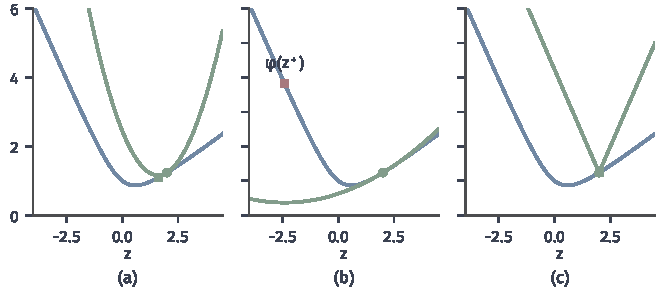
\includegraphics[width=112mm]{figures/05-optimization/04-block-optimization/matplotlib/block-bsum-conditions/figure.pdf}
  \caption{块上界的三个条件。蓝色是条件函数$\varphi(z)=\sqrt{1+z^2}-z/2$，绿色是模型，绿点是当前点$z=2$，方块是模型最小点上原函数的值。(a)二次上界满足全部条件。(b)二阶Taylor模型不是上界，最小点走得太远，红色方块处的目标值反而升高。(c)带尖角的上界满足上界与相等条件，但方向导数不一致，最小点就是当前点。}
  \label{fig:block-bsum-conditions}
\end{BookInlineFigure}

\paragraph{上界要覆盖全部允许变化}
上界必须在整个$\bm{C}_J$上成立，因为子问题的解可能落在$\bm{C}_J$的任何位置。只在当前点附近成立的局部近似，比如(b)中的Taylor模型，不能用式~\eqref{eq:block-bsum-descent}这条链。

这时要另外控制接受：用线搜索沿模型方向检验真实目标，或用第~\ref{chap:trust-region}章的信赖域限制模型的使用范围。这两种机制是用额外的函数值检验来替代上界保证。

\subsection{上界的构造}
\label{sec:block-bsum-construction}

\paragraph{一阶上界}
第一种构造用光滑项的二次上界。设$F=f$可微，且满足定义~\ref{def:block-smooth}，取
\begin{equation}
 u_J(\bm{z};\bm{y})=f(\bm{y})+\langle\nabla_Jf(\bm{y}),\bm{z}-\bm{y}_J\rangle+\frac{L_J}{2}\lVert\bm{z}-\bm{y}_J\rVert_2^2 .
 \label{eq:block-ub-quadratic}
\end{equation}
上界条件来自式~\eqref{eq:block-quadratic-upper}，相等和一阶条件可以直接核对。子问题有闭式解，难解的条件函数换成了一个球形的二次函数。

再看前面的条件函数$\varphi(z)=\sqrt{1+z^2}-z/2$，$L_J=1$，$z=2$。原条件问题要解$z/\sqrt{1+z^2}=\tfrac12$，模型的最小点却只要一次减法：
\[
 z^{+}=2-\varphi'(2)\approx1.606 .
\]
下降链~\eqref{eq:block-bsum-descent}在这里的数值是
\[
 \varphi(z^{+})\approx1.089\leq u(z^{+})\approx1.158\leq u(2)=\varphi(2)\approx1.236 .
\]

\paragraph{保留原目标加距离项}
第二种构造不改变原条件函数，只在外面加一个二次距离项，$\beta>0$：
\begin{equation}
 u_J(\bm{z};\bm{y})=F\bigl(\bm{y}+\bm{U}_J(\bm{z}-\bm{y}_J)\bigr)+\frac{\beta}{2}\lVert\bm{z}-\bm{y}_J\rVert_2^2 .
 \label{eq:block-ub-proximal}
\end{equation}
距离项非负，所以它不低于条件函数；在当前点距离项为零，两者相等；距离项在当前点的方向导数为零，所以一阶条件也成立。这种构造不简化子问题，但改善了子问题的结构。

二次项的作用有两种。一是控制曲率：条件函数的曲率有负的下界$-\sigma$时，取$\beta>\sigma$，子问题就变成强凸的。二是改善唯一性：第~\ref{sec:block-convergence}小节的极限分析要求子问题的解唯一，距离项能把多解的子问题变成单解。

图~\ref{fig:block-bsum-constructions}(b)取$\varphi(z)=(z^2-1)^2$，它有两个最小点$\pm1$，曲率下界是$-4$。在$z=0.3$处取$\beta=10$，模型变成强凸，只有一个最小点，约在$0.44$。

\begin{BookInlineFigure}
  \centering
  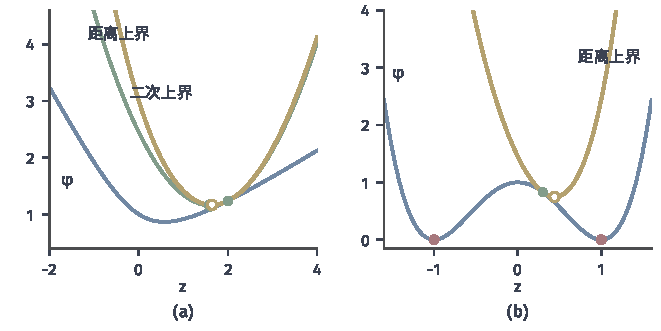
\includegraphics[width=112mm]{figures/05-optimization/04-block-optimization/matplotlib/block-bsum-constructions/figure.pdf}
  \caption{两种块上界的构造。(a)$\varphi(z)=\sqrt{1+z^2}-z/2$（蓝）在$z=2$处的二次上界（绿，$L_J=1$）和保留原函数的距离上界（黄，$\beta=1$），空心点是各自的最小点。(b)非凸函数$\varphi(z)=(z^2-1)^2$有两个最小点（红），在绿点$z=0.3$处加上$\tfrac{10}{2}(z-0.3)^2$后，距离上界（黄）只有一个最小点（空心）。}
  \label{fig:block-bsum-constructions}
\end{BookInlineFigure}

\paragraph{通向块邻近模型}
第三种构造介于两者之间。设目标$F=f+\sum_Jg_J$，光滑项$f$用二次上界代替，可分的非光滑项$g_J$原样保留。这样子问题既保留了$g_J$的结构，又不必处理$f$的复杂形式，这就是第~\ref{sec:block-bpg}节的块邻近模型。

\subsection{与其他块方法的关系}
\label{sec:block-bsum-relations}

把各种更新放进BSUM的框架，能看清谁是谁的特例，也能看清谁不是。图~\ref{fig:block-relations}汇总了这些关系。

\begin{BookInlineFigure}
  \centering
  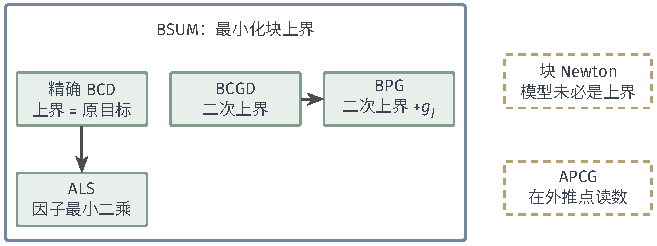
\includegraphics[width=110mm]{figures/05-optimization/04-block-optimization/tikz/block-relations/figure.pdf}
  \caption{BSUM与其他块方法的关系。实线框内是满足块上界条件的更新：精确BCD的上界是条件函数本身，BCGD用二次上界，BPG再保留可分项$g_J$，ALS是因子问题上的精确BCD。黄色虚线框的两种方法一般不满足这些条件，不能未经核验就使用BSUM的下降与收敛保证。}
  \label{fig:block-relations}
\end{BookInlineFigure}

\paragraph{属于BSUM的情形}
当$u_J$就是条件函数时，式~\eqref{eq:block-bsum}就是精确BCD。取式~\eqref{eq:block-ub-quadratic}得到BCGD。下一节的块邻近梯度取光滑部分的二次上界加$g_J$。ALS是因子问题上的精确求解，所以也在框内，但它的关键在于因子结构带来的闭式最小二乘，这一点并不是BSUM框架提供的。

这些关系是按模型的选择和问题的结构形成的交叉，而不是一棵分类树。同一个算法可以从几种角度描述。比如对二次目标，式~\eqref{eq:block-ub-quadratic}取$L_J=Q_{J,J}$（单坐标）时，BCGD和精确BCD就是同一个更新。

\paragraph{不属于BSUM的情形}
一般的块Newton模型不是上界，图~\ref{fig:block-bsum-conditions}(b)已经说明，它需要线搜索或信赖域来保证接受。只有当二阶模型恰好被改造成上界时（比如把Hessian主子矩阵换成一个不小于真实Hessian的矩阵），才回到BSUM。

APCG的模型建立在外推点上，式~\eqref{eq:block-bsum-descent}这样的单调链不成立，手算例子中目标值也确实上升过。它的收敛结论靠的是辅助序列的递推，定理~\ref{thm:block-apcg}不能由BSUM的结论推出。
